\documentclass[10pt, compress]{beamer}

\usepackage{
    algorithm,algorithmic,amsfonts,amsmath,amssymb,bm,booktabs,color,
    enumerate,graphicx,hyperref,microtype,multicol,natbib,nicefrac,url
}
\usepackage[T1]{fontenc}
\usepackage[utf8]{inputenc}

\newcommand{\todo}[1]{\noindent\textbf{\textcolor{red}{(TODO) #1\\}}}

\newcommand{\MDP}{M}
\newcommand{\States}{\mathcal{S}}
\newcommand{\Actions}{\mathcal{A}}
\newcommand{\cost}{C}
\newcommand{\initstatedist}{\rho}
\newcommand{\discount}{\gamma}
\newcommand{\numsamp}{N}
\newcommand{\horizon}{T}
\newcommand{\dynamics}{p}
\newcommand{\policyparams}{\theta}
\newcommand{\policy}{\pi}
\newcommand{\state}{\mathbf{s}}
\renewcommand{\action}{\mathbf{a}}
\newcommand{\costsample}{c}
\newcommand{\policyobj}{\eta}
\newcommand{\dynmodel}{\hat{\dynamics}}
\newcommand{\costmodel}{\hat{\cost}}
\newcommand{\isdmodel}{\hat{\rho}}
\newcommand{\dynmat}{\mathbf{F}}
\newcommand{\dyncovar}{\Sigma}
\newcommand{\costmat}{\mathbf{C}}
\newcommand{\costvec}{\mathbf{c}}
\newcommand{\K}{\mathbf{K}}
\renewcommand{\k}{\mathbf{k}}
\newcommand{\polcovar}{\mathbf{S}}
\newcommand{\latent}{\mathbf{x}}
\newcommand{\traj}{\tau}
\newcommand{\polstepsize}{\epsilon_p}
\newcommand{\modelstepsize}{\epsilon_m}
\newcommand{\R}{\mathbb{R}}
\newcommand{\N}{\mathcal{N}}
\newcommand{\W}{\mathcal{W}}
\renewcommand{\L}{\mathcal{L}}
\newcommand{\E}{\mathbb{E}}
\newcommand{\I}{\mathbb{I}}
\newcommand{\KL}{\text{KL}}
\newcommand{\model}{\mathcal{M}}
\newcommand{\dataset}{\mathcal{D}}
\DeclareMathOperator*{\argmin}{argmin}
\DeclareMathOperator*{\argmax}{argmax}
\newcommand{\colvec}[2][.67]{%
  \scalebox{#1}{%
    \renewcommand{\arraystretch}{.67}%
    $\begin{bmatrix}#2\end{bmatrix}$%
  }
}
\newcommand{\trajectory}{\left[\state_0,\action_0,\ldots,\state_\horizon,\action_\horizon,\state_{\horizon + 1}\right]}
\newcommand{\costtrajectory}{\left[\state_0,\action_0,\costsample_0\ldots,\state_\horizon,\action_\horizon,\costsample_\horizon,\state_{\horizon + 1}\right]}
\newcommand{\latenttrajectory}{\left[\latent_0,\action_0,\ldots,\latent_\horizon,\action_\horizon,\latent_{\horizon + 1}\right]}

\usetheme{metropolis}           % Use metropolis theme

\PassOptionsToPackage{export}{adjustbox}
\usetikzlibrary{fit, positioning}
\usepackage{bm}
\usepackage[mode=buildnew]{standalone}
%\usepackage[export]{adjustbox}
\usepackage{booktabs}
\usepackage[scale=2]{ccicons}
\usefonttheme[onlymath]{serif}
\usepackage{pdfpcnotes}

%\usemintedstyle{trac}

\title{Model learning with structured latent representations}
\subtitle{}
\date{\today}
\author{Sharad Vikram}
\institute{UCSD}

%\setcounter{tocdepth}{1}

\begin{document}

\begin{frame}
	\titlepage
\end{frame}

\section{Background}

\subsection{Probabilistic graphical models}

%\begin{frame}{Random variables}
%A random variable is a quantity with uncertainty associated with it.
%\pause

%Every random variable is associated with a \emph{distribution}
%over its possible values, for example

%\begin{align*}
%x \sim \N(0, 1)
%\end{align*},

%and a probability distribution function $p(x)$.

%\end{frame}

\begin{frame}{Probabilistic graphical models}
	A probabilistic graphical model (PGM)
	is a graphical representation of a joint distribution
	over several random variables.
	\pause

	For example, a possible graph for variables $x, y$ and $z$ is
	\begin{center}
		\includestandalone[width=0.3\textwidth]{tikz/pgm}
	\end{center}
	\pause
	The joint distribution factorizes as
	\begin{align*}
		p(x, y, z) = p(x)p(y | x)p(z | x, y)
	\end{align*}
\end{frame}

\begin{frame}{Bayesian inference}
	Bayesian inference allows us to
	compute probability distributions
	after observations have been made.

	\pause

	\begin{center}
		\includestandalone[width=0.3\textwidth]{tikz/pgm-obs}
	\end{center}
	\pause
	We are interested in the posterior distribution $p(x, y | z)$

	\pause
	This can be computed via Bayes rule:
	\begin{align*}
		p(x, y | z) = \frac{p(x, y, z)}{p(z)} = \frac{p(x)p(y | x)p(z | x, y)}{\int p(x)p(y | x)p(z | x, y)dx dy}
	\end{align*}
\end{frame}

\begin{frame}{Example PGM}
	\textbf{Latent variable model}: Gaussian mixture model
	\begin{center}
		\includestandalone[width=0.3\textwidth]{tikz/gmm}
	\end{center}

	\pause
	\textbf{Local variables}: $\{z_i\}_{i=1}^N$

	\pause
	\textbf{Global variables}: $\mu, \pi$

\end{frame}

\begin{frame}{Conjugacy}
	\metroset{block=fill}
	\begin{block}{Conjugate}
		Two random variables $x$ and $y$ whose distribution is
		\begin{align*}p(x, y) = p(x)p(y | x)\end{align*} are said to be
			\emph{conjugate} if the posterior $p(x | y)$
		is in the same family of distributions as $p(x)$.
	\end{block}
	\pause
	Examples of conjugate distributions:
	\begin{itemize}
		\item Normal/normal
			\pause
		\item Normal-inverse-wishart(NIW)/normal
			\pause
		\item Dirichlet/multinomial
	\end{itemize}
\end{frame}

\begin{frame}{Algorithms for inference}
	Depending on the structure of the graphical model
	and conjugacy of the variables, computing the posterior distribution
	can be easy, or very hard!

	\pause
	Possible ways:
	\begin{itemize}
		\item<2-> Compute posterior analytically
			\pause
		\item<3-> Sampling (MCMC, Gibbs sampling)
			\pause
		\item<4-> Expectation-maximization
			\pause
		\item<5->\alert<6->{Variational inference}
	\end{itemize}
	\pause
	PGMs offer interpretability and quantifiable uncertainty,
	but often don't scale well with data
	and can be underexpressive.
\end{frame}

\subsection{Model learning}

\begin{frame}{Model learning}
	Consider an agent in a system,
	and a set of its possible actions.
	\begin{center}
		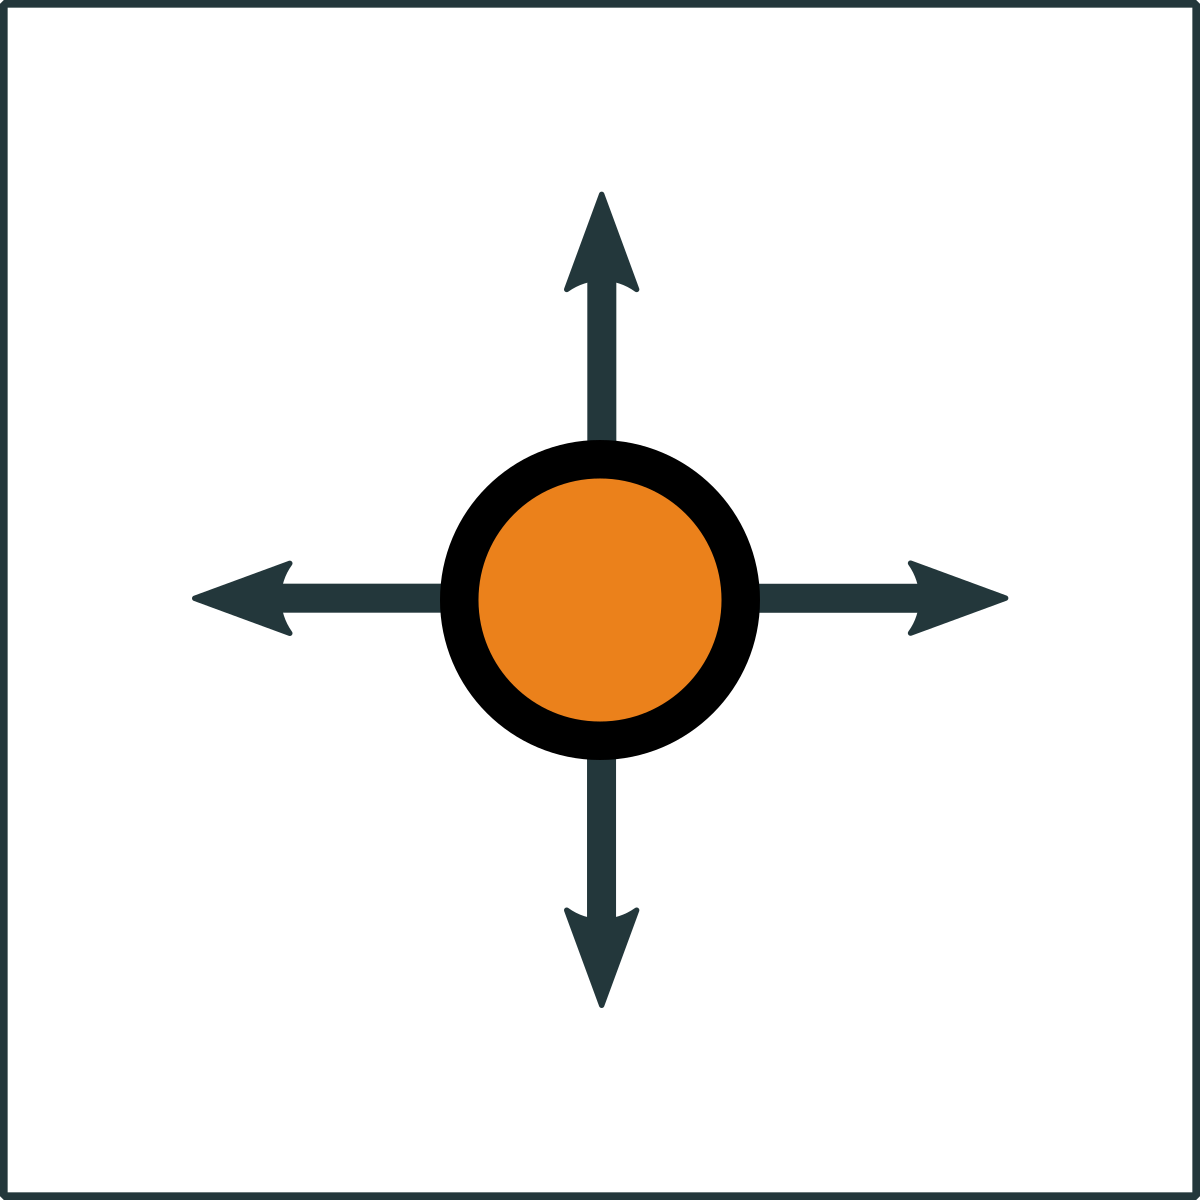
\includegraphics[width=0.5\textwidth]{img/agent-env-1.png}
	\end{center}
	\pause
	Model learning is the problem of estimating the dynamics of the system
	when we don't know it beforehand.
\end{frame}

\begin{frame}{Model learning}
	Formally, consider an agent in a system with state space $\mathcal{S}$
	with action space $\mathcal{A}$ with underlying dynamics 
	function $p(s_{t + 1} | s_t, a_t)$.

	We are interested in learning an approximate dynamics function
	\begin{align*}\hat{p}(s_{t + 1} | s_t, a_t)\end{align*}
		from a dataset of trajectories \begin{align*}\bm{\tau} = \{(s^{(i)}_0, a^{(i)}_0, s^{(i)}_1, a^{(i)}_1, \ldots, s^{(i)}_T)\}_{i = 1}^N\end{align*}
\end{frame}

\begin{frame}{Bayesian linear dynamical system}
	\pnote{Talk about conjugacy}
	A simple assumption: \textbf{Bayesian linear dynamical system} (LDS)
	\begin{alignat*}{3}
		\mu_{\isdmodel},\Sigma_{\isdmodel}&\sim\mathcal{NIW}(\Psi,\nu,\mu_0,\kappa)\,,~~~\dynmat,\dyncovar&&\sim\mathcal{MNIW}(\Psi,\nu,\bm{M}_0,\bm{V})\,,\\
		\state_0~|~\mu_{\isdmodel},\Sigma_{\isdmodel}&\sim\N(\mu_{\isdmodel}, \Sigma_{\isdmodel})\,,~~~~~\state_{t+1}~|~\state_t,\action_t&&\sim\N\left(\dynmat\begin{bmatrix}\state_t\\\action_t\end{bmatrix},\dyncovar\right) \textrm{ for } t \in [0,\ldots,\horizon]
	\end{alignat*}
	\pause
	\centering
	\includestandalone[width=0.5\textwidth]{tikz/blds}

	\pause
	We are interested in the posterior distribution 
	$
	p(\mu_\isdmodel, \Sigma_\isdmodel, \dynmat, \dyncovar | {s_0, a_0, \ldots, s_T})
	$
	which can be computed analytically.
\end{frame}

\subsection{Variational inference}
\begin{frame}{Variational inference at a high level}
	%For graphical models where we can't compute
	%the posterior analytically, \textbf{variational inference}
	%is a viable approach.

	\pause
		Consider a latent variable model with global variables
		$\theta$, local variables $z$ and observations $x$. Our desired
		posterior is $p(\theta, z | x)$

		\pause
		\textbf{Strategy}: convert inference into optimization
		\begin{itemize}
				\pause
			\item Instantiate \emph{variational distribution} $q_\phi(\theta, z)$
				where $\phi$ are free parameters
				\pause
			\item Define loss $\textrm{KL}(q_\phi(\theta, z)\|p(\theta, z | x))$
				\pause
			\item Minimize loss $\phi^* = \argmin_\phi \textrm{KL}(q_\phi(\theta, z)\|p(\theta, z | x))$
		\end{itemize}
		\pause
		If $q(\theta, z)$ is sufficiently expressive,
		it can approximate $p(\theta, z | x)$ quite well.
\end{frame}

\begin{frame}{KL-divergence}
	Kullback-Leibler (KL) divergence
	is a measure of how far one probability distribution
	is from another.

	\pause
	For distributions $q(x)$ and $p(x)$,
	\begin{align*}
		\textrm{KL}(q(x)\|p(x)) = \int q(x)\log \frac{q(x)}{p(x)}dx
	\end{align*}

	\pause
	\textbf{Properties:}
	\begin{itemize}
		\item $\textrm{KL}(q(x)\|p(x)) = 0$ if $q(x) = p(x)$.
		\item Asymmetric
	\end{itemize}

\end{frame}

\begin{frame}{Evidence lower bound}
	In general, we cannot even compute $KL(q(\theta, z)\|p(\theta, z | x))$
	because
	we don't know the posterior $p(\theta, z | x)$.

	\pause
	We can rewrite the KL divergence as
	\begin{align*}
		\KL(q(\theta, z)\|p(\theta, z|x)) &= \int q(\theta, z)\log\frac{q(\theta, z)}{p(\theta, z | x)}d\theta, z \\
		%&= \int q(\theta, z) \left(\log q(\theta, z) - \log p(\theta, z | x)\right)d\theta, z \\
		%&= \int q(\theta, z) \left(\log q(\theta, z) - \log \frac{p(\theta, z, x)}{p(x)}\right)d\theta, z \\
		%&= \int q(\theta, z) \left(\log q(\theta, z) - \log p(\theta, z, x) + \log p(x)\right)d\theta, z \\
							&= \log p(x) - \E_{q(\theta, z)}\left[\log\frac{p(x, \theta, z)}{q(\theta, z)}\right]
	\end{align*}

	\pause
	and maximize the \emph{evidence lower bound} (ELBO)
	\begin{align*}
		\L[q(\theta, z)] &= \E_{q(\theta, z)}\left[\log\frac{p(x, \theta, z)}{q(\theta, z)}\right]
	\end{align*}
\end{frame}

\begin{frame}{Variational inference for PGMs}
	For a general graphical model
	with variable set $\mathbf{X} = \{x_1, x_2, \ldots\}$
	we have joint distribution
	\begin{align*}
		p(\mathbf{X}) = \prod_i p(x_i | \textrm{pa}_i)
	\end{align*}
	where $\textrm{pa}_i$ are the parents of node $x_i$
	in the graph.


	\pause
	Let the set $\mathbf{H}$ be
	all unobserved variables and $\mathbf{V}$ be the observed.


	\pause
	We are interested in the posterior $p(\mathbf{H} | \mathbf{V})$
	and use variational distribution 
	\begin{align*}
		q(\mathbf{H}) = \prod_i q(\mathbf{H}_i)
	\end{align*}

	\pause
	This is called the \emph{mean-field} assumption.

\end{frame}

\begin{frame}{Variational inference for PGMs (cont.)}
	The ELBO is now
	\begin{align*}
		\L[q(\mathbf{H})] &= \E_{q(\mathbf{H})} \left[\log\frac{p(\mathbf{H}, \mathbf{V})}{q(\mathbf{H})}\right] \\
											&= \int\prod_i q(\mathbf{H}_i) \left(\log p(\mathbf{H}, \mathbf{V}) - \log \prod_i q(\mathbf{H}_i)\right)d\mathbf{H}\\
											&= \int q(\mathbf{H}_j) \left(\int \log p(\mathbf{H}, \mathbf{V})\prod_{i \neq j}q(\mathbf{H}_i)d\mathbf{H}_i \right)d\mathbf{H}_j \\&- \int q(\mathbf{H}_j)\log q(\mathbf{H}_j)d \mathbf{H}_j + \textrm{const.}\\
											&= \int q(\mathbf{H}_j)\log \tilde{q}(\mathbf{H}_j, \mathbf{V})d \mathbf{H}_j- \int q(\mathbf{H}_j)\log q(\mathbf{H}_j)d \mathbf{H}_j  + \textrm{const.} \\
											&= -\KL(q(\mathbf{H}_j)\|\tilde{q}(\mathbf{H}_j, \mathbf{V}))  + \textrm{const.}
	\end{align*}
	where 
	\begin{align*}
		\log\tilde{q}(\mathbf{H}_j, \mathbf{V}) = \E_{i \neq j}\left[\log p(\mathbf{H}, \mathbf{V})\right] + \textrm{const.}
	\end{align*}

\end{frame}

\begin{frame}{Optimizing a single factor}
	We can isolate a single factor for each hidden node in the graph $\mathbf{H}_j$.
	This makes optimizing a single variational factor easy!
	\pause
	\begin{align*}
		\L[q(\mathbf{H})] &= \KL(q(\mathbf{H}_j)\|\tilde{q}(\mathbf{H}_j, \mathbf{V}))  + \textrm{const.}
	\end{align*}
	\pause
	For a single factor $q(\mathbf{H}_j)$, this equation is minimized
	when $q(\mathbf{H}_j) = \tilde{q}(\mathbf{H}_j, \mathbf{V})$.

	\pause
	Furthermore, 
	\begin{align*}
		\log\tilde{q}(\mathbf{H}_j, \mathbf{V}) = \E_{i \neq j}\left[\log p(\mathbf{H}, \mathbf{V})\right] + \textrm{const.}
	\end{align*}
	is a function of only factors other than $q(\mathbf{H}_j)$  and observed data.

	\pause
	\metroset{block=fill}
	\begin{block}{Mean-field variational inference}
		Until converged,
		for each factor $q(\mathbf{H}_j)$,
		hold factors $q(\mathbf{H}_{i \neq j})$ constant and
		set $q(\mathbf{H}_j) = \tilde{q}(\mathbf{H}_j, \mathbf{V})$.
	\end{block}
\end{frame}

\begin{frame}{Conjugate-exponential graphical models}
	If our PGM is \emph{conjugate-exponential},
	where every node belongs in the exponential
	family of distributions, and is conjugate w.r.t. its parents,
	\begin{align*}
		\log\tilde{q}(\mathbf{H}_j, \mathbf{V}) = \E_{i \neq j}\left[\log p(\mathbf{H}, \mathbf{V})\right] + \textrm{const.}
	\end{align*}

	can be calculated in closed form!

	\pause
	An exponential family distribution is one that can be written in the following form:
	\begin{align*}
		p(x | \theta) = h(x) \exp \left\{\left\langle \eta_x(\theta), t_x(x)\right\rangle - \log Z(\eta(\theta))\right\}
	\end{align*}
	with 
	\begin{itemize}
			\pause
		\item $h(x)$: base measure
			\pause
		\item $\eta_x(\theta)$: natural parameter
			\pause
		\item $t_x(x)$: sufficient statistic
			\pause
		\item $\log Z(\eta_x(\theta))$: log-partition function
	\end{itemize}
\end{frame}

\begin{frame}{Variational message passing}
	We now return to graphs! If we assume a mean-field
	variational distribution and our PGM is conjugate-exponential,
	we get a very elegant graph algorithm, called \emph{variational message passing} (VMP) \cite{vmp}.

	\begin{center}
		\includegraphics<1>[width=0.5\textwidth]{img/vmp-1}
		\includegraphics<2>[width=0.5\textwidth]{img/vmp-2}
		\includegraphics<3>[width=0.5\textwidth]{img/vmp-3}
		\includegraphics<4>[width=0.5\textwidth]{img/vmp-4}
	\end{center}

\end{frame}

\begin{frame}{Messages}
	Remember that $\eta_j$ is the natural parameter of the distribution $q(\mathbf{H}_j)$.
	\pause
	The message from a parent $Y$ to a child $X$ is
	\begin{align*}
		m_{Y \rightarrow X} = f(\eta_Y)
	\end{align*}
		\pause
	The message from a child $X$ to a parent $Y$ is
	\begin{align*}
		m_{X \rightarrow Y} = g(\eta_X, \{m_{i \rightarrow X}\}_{i \in \textrm{cp}_Y})
	\end{align*}

	\pause
	In conjugate-exponential PGMs, messages can be computed in closed-form.
\end{frame}

\begin{frame}{Summary of VMP}
	\textbf{Setup:} Conjugate-exponential graphical model

	\pause
	\textbf{Problem:} Compute posterior $p(\mathbf{H} | \mathbf{V})$, approximated with $q(\mathbf{H}) = \prod_j q(\mathbf{H}_j)$

	\pause
	\textbf{Solution:} Until converged, for each hidden node $\mathbf{H}_j$:
	\begin{enumerate}
			\pause
		\item Collect messages from children and parents
			\pause
		\item Compute updated distribution parameters from messages
	\end{enumerate}

	\pause
	\textbf{Benefits:} efficient, simple, can incorporate mini-batches (stochastic variational inference)

	\pause
	\textbf{Drawbacks:} can be underexpressive (conjugate-exponential requirement)
\end{frame}

\section{Structured variational autoencoder}

\subsection{Model learning}

\begin{frame}{Model learning}
	Recall the model learning problem.
	\pause
	\begin{center}
		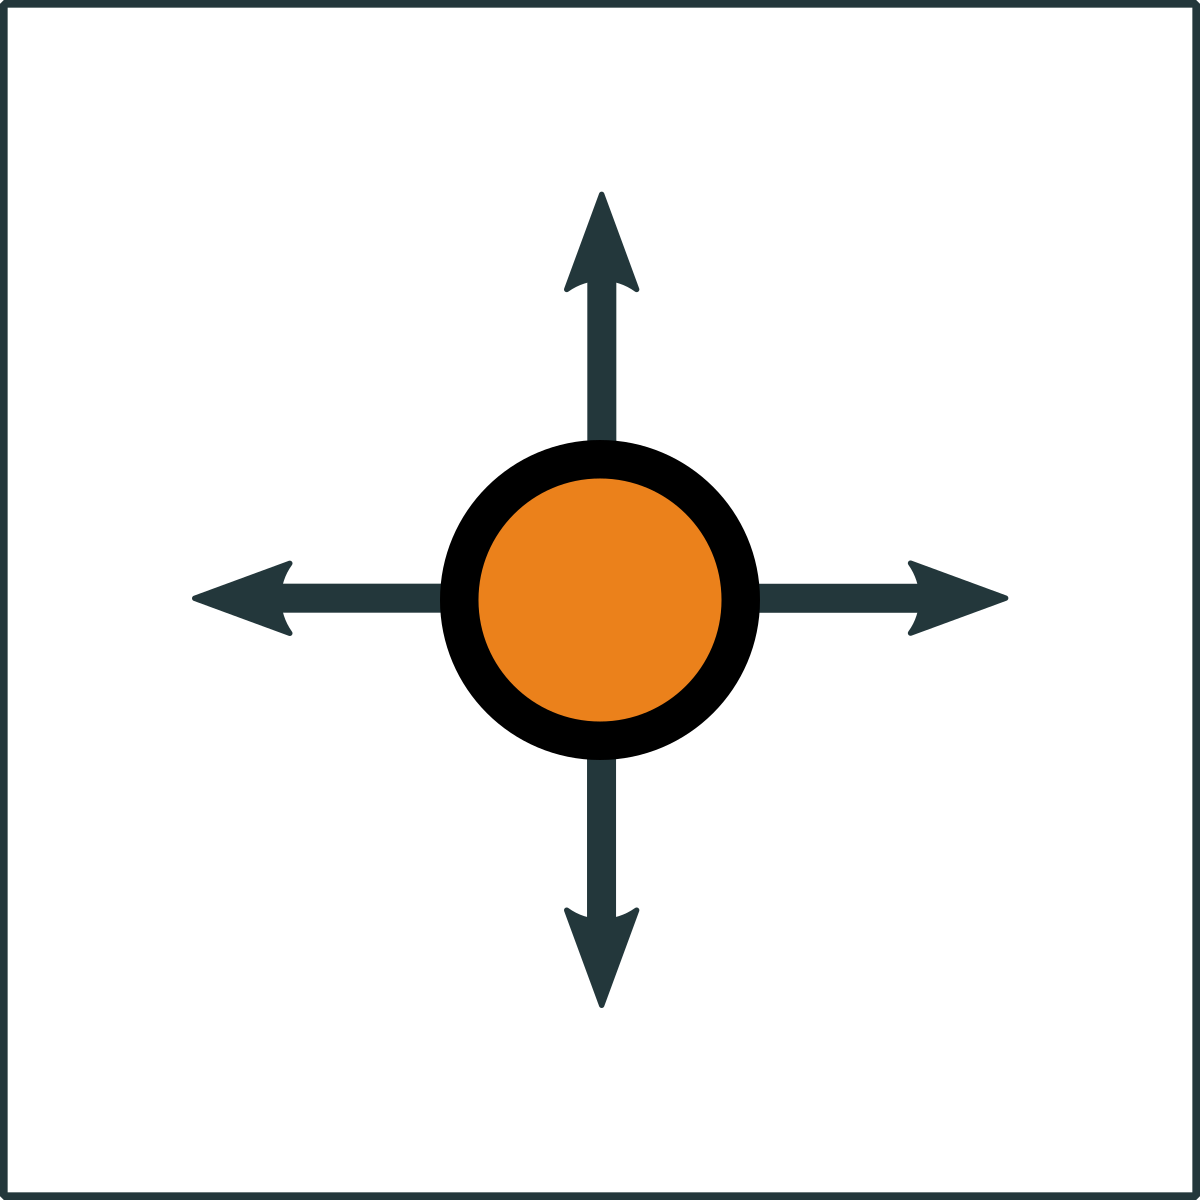
\includegraphics[width=0.3\textwidth]{img/agent-env-1.png}
	\end{center}

	\pause
	\centering
	\includestandalone[width=0.4\textwidth]{tikz/blds}
\end{frame}

\begin{frame}{Adding expressivity}
	One way of making the Bayesian LDS more expressive
	is to add a observation model.

	\pause

	\centering
	\includestandalone[width=0.4\textwidth]{tikz/lblds}

	\pause

	What if this observation model was a neural network?
\end{frame}

\begin{frame}{Structured variational autoencoder}
	We augment the Bayesian LDS with a neural network observation model.
	\pause
	\begin{alignat*}{3}
		\mu_{\isdmodel},\Sigma_{\isdmodel}&\sim\mathcal{NIW}(\Psi,\nu,\mu_0,\kappa)\,,~~~\dynmat,\dyncovar&&\sim\mathcal{MNIW}(\Psi,\nu,\bm{M}_0,\bm{V})\,,\label{eq:ldssvae-start}\\
		\latent_0~|~\mu_{\isdmodel},\Sigma_{\isdmodel}&\sim\N(\mu_{\isdmodel}, \Sigma_{\isdmodel})\,,~~~~~\latent_{t+1}~|~\latent_t,\action_t&&\sim\N\left(\dynmat\begin{bmatrix}\latent_t\\\action_t\end{bmatrix},\dyncovar\right) \textrm{ for } t \in [0,\ldots,\horizon]\,,\\
			\state_t~|~\latent_t&\sim\N\left(\mu_\gamma(\latent_t),\Sigma_\gamma(\latent_t)\right) \text{ for } t \in &&[0,\ldots,\horizon]
	\end{alignat*}
	where $\mu_\gamma(\latent_t)$ and $\Sigma_\gamma(\latent_t)$ are both neural networks parametrized by $\gamma$.
	This model is called a structured variational autoencoder (SVAE) \cite{svae}.

	\pause
	\textbf{But what does it do?}
\end{frame}

\begin{frame}{Inference in SVAE}
	First of all, a neural network is neither conjugate nor exponential.
	How do we perform inference?

	\pause
	\textbf{Strategy:} Run VMP, but use ``fake'' messages for the neural network observation model.

	\begin{center}
		\includegraphics<2>[width=0.15\textwidth]{img/vmp-svae-1}
		\includegraphics<3>[width=0.15\textwidth]{img/vmp-svae-2}
		\includegraphics<4>[width=0.15\textwidth]{img/vmp-svae-3}
	\end{center}

\end{frame}


\begin{frame}{Messages in SVAE}
	The message from a \textbf{non-conjugate, non-exponential family} observation $X$ to a parent $Y$ is
	\begin{align*}
		m_{X \rightarrow Y} = r_\xi(t_X(X))
	\end{align*}
	where $r_\xi$ is a neural network whose output
	is the same shape of a message from a conjugate-exponential child.

	\pause
	\metroset{block=fill}
	\begin{block}{Inference in a SVAE}
		\begin{enumerate}
			\item For a data $\tau = \{s_0, a_0, s_1, a_1, \ldots, s_T\}$,
				perform VMP using SVAE messages
			\item Compute the ELBO $\L[q(\{x_i\}_{i = 1}^T, \mu_{\isdmodel}, \Sigma_{\isdmodel}, \dynmat, \dyncovar)]$
			\item Update neural networks with $\nabla_{\gamma, \xi} \L[q(\{x_i\}_{i = 1}^T, \mu_{\isdmodel}, \Sigma_{\isdmodel}, \dynmat, \dyncovar)]$
			\item Update global parameters ($\mu_{\isdmodel}, \Sigma_{\isdmodel}, \dynmat, \dyncovar$) with natural gradients
		\end{enumerate}
	\end{block}
\end{frame}

\begin{frame}{Autoencoding}
	How is a SVAE an \emph{autoencoder}?

	\begin{center}
		\includestandalone[width=0.4\textwidth]{tikz/lblds}
	\end{center}

	\pause
	We have two neural networks:
	\begin{enumerate}
			\pause
		\item $r_\xi(s)$: recognition network, takes real data and ``encodes'' it
			\pause
		\item $\mu_\gamma(x), \Sigma_\gamma(x)$: observation network, takes latent data and ``decodes'' it
	\end{enumerate}
\end{frame}

\section{Conclusion}

\subsection{Applications}
\begin{frame}{Why SVAE?}
	The SVAE naturally applies to scenarios where there is already a tractable PGM.

	\pause
	\begin{center}
		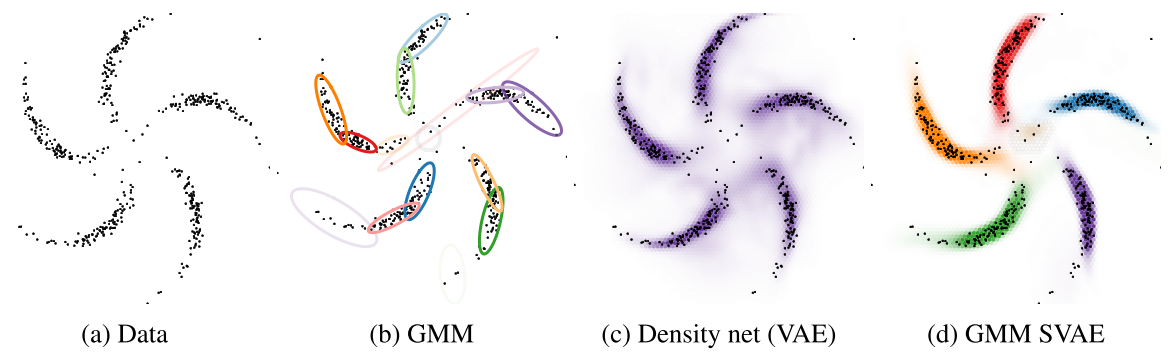
\includegraphics[frame,width=\textwidth]{img/svae-example}
	\end{center}

	\pause
	In this scenario, the SVAE enables modeling non-Gaussian cluster shapes \cite{svae}.
\end{frame}

\subsection{Current work}
\begin{frame}{Current work}
	One idea I am currently working on is using the SVAE to learn
	latent models to be used in reinforcement learning\footnotemark.

	\pause
	\textbf{General approach:}
	\begin{itemize}
		\item Learn a latent LDS
		\item Use MPC to control an agent in the latent space
	\end{itemize}

	\pause
	\textbf{Benefits of this approach:}
	\begin{itemize}
			\pause
		\item We can learn simple dynamics even with camera data
			\pause
		\item Model-based RL tends to be more sample efficient
			\pause
	\end{itemize}
	\pause
	\alert{Demo}
	\footnotetext[1]{Joint work with Marvin Zhang from UC Berkeley}
\end{frame}

\begin{frame}[standout]
	Questions?
\end{frame}

\appendix
\begin{frame}[allowframebreaks]{References}
	\bibliography{main}
	\bibliographystyle{unsrt}
\end{frame}


\end{document}
